\chapter{Methods}
\label{chap:methods}
\minitoc

\section{Dataset}
In this section, we will describe the dataset used in this work to train, test and validate the models. 
\par We used open-source data published on the \cite{EDP} \emph{OpenData} web platform and made available for research purposes. 
The data was collected from the SCADA systems of five different Vestas wind turbines (Turbine 01, 06, 07, 09 and 11) in the same wind park between the years 2016 and 2017 
and is made up of the following four subsets: \emph{Signals, Logs, Failures and Metmast}. We will, however, only describe three sets since \emph{Metmast} was not used in this work.
\subsection{Signals}
 The \emph{Signals} dataset contains 10-min-averaged data collected from the wind turbines' sensors installed at the major components (e.g., gearbox, generator, transformer,..) 
 and power meters to measure temperatures, angles, wind and rotational speeds, power production,... 
 This dataset was the most crucial for this work since it provides information that reflects the status of the turbine operation which is needed to perform 
 automated condition monitoring and predictive maintenance.\\
 Table \ref{tab:signals} shows a sample of the 81 signals included in this dataset.
 \begin{table}
        \centering
    \begin{tabular}{ | m{12em} | m{8cm} | }
    \hline
         \multicolumn{1}{|c|}{\textbf{Type of signal}} & \multicolumn{1}{c|}{\textbf{Signals}} \\
         \hline
         Average temperature (\degree C) & Generator, Generator bearings, Hydraulic group oil, Gearbox oil, Gearbox bearing on the high-speed shaft, 
         Nacelle, HV transformer, Ambient temperature,..  \\
         \hline
         Average production value & Active power (Wh), Reactive power (VArh), Power according to grid (kW),.. \\
    \hline
    \end{tabular}
    \caption{Sample signals found in the Signals dataset}
        \label{tab:signals}
\end{table}
 \subsection{Logs}
  In this dataset, events logged by the SCADA system are collected in non-fixed intervals. The events recorded by the system are divided into three categories: Alarm log, 
  Warning log and Operation and System log. According to the VestasOnline Enterprise user manual \cite{voe},  alarms are system notifications that alert operators to 
  an error scenario that has forced a wind turbine to cease normal operation and transition to one of three operational states: Pause, Stop, or 
  Emergency (one of the following three acknowledgments is needed to resume operation: Local acknowledgment 
  from the controller unit of the turbine, Remote acknowledgment from VestasOnline®, or Automatic acknowledgment), 
  whereas warnings are system messages that indicate an irregularity that requires attention but does not cause the turbine 
  to immediately cease normal operation and exit the Run state.
  \begin{table}
          \centering
      \begin{tabular}{|c|c|}
      \hline
          \textbf{Type of log event} & \textbf{Sample log event}  \\
          \hline
          \multirow{2}{12em}{\centering Alarm log} & \emph{"High temperature brake disc"} \\
          & \emph{"High pres offlin:\_\_\_\_RPM/ \_\_\_\degree C"} \\
          \hline
          \multirow{2}{12em}{\centering Warning log} & \emph{"Yaw Position is changed: \_\_\degree"} \\
          & \emph{"Low Battery Nacelle"} \\
          \hline
          \multirow{2}{12em}{\centering Operation and System log} & \emph{"External power ref.:\_\_\_\_kW"} \\
          & \emph{"GearoilCooler \_, gear: \_\_\_\degree C"} \\
      \hline
      \end{tabular}
      \caption{Sample log events found in the Logs dataset}
          \label{tab:metrics}
  \end{table}
\subsection{Failures}
  The Failures dataset contains the history of failures, inspections, or maintenance that occurred in the turbines and was manually recorded by technicians. 
  Each record reports the time of the event, component (e.g., Generator, Hydraulic group,..), and a text description of the failure 
  or event (e.g., "Generator replaced", "Oil leakage in Hub",..).\\ 
  This dataset was used in backtesting to validate the models' capability of detecting failures early.


\section{Machine learning models}
In this section, we will demonstrate the architecture of the machine learning models used in our experiments.

\subsection{Linear regression}
  Sir Francis Galton proposed the idea of linear regression in 1894 \cite{Natural_Inheritance}.
  Linear regression is used for analyzing the linear relationship between one or more independent variables (X) and a dependent variable (Y).
  The dependent variable Y must be continuous, whereas the independent variables can be continuous or categorical. \\
  When the relationship between the dependent variable and the independent variables is assumed to be linear and there are a small number of independent variables, 
  linear regression is usually used. Linear regression is easy to use and understand, and it can be used to make predictions or find relationships between variables.\\
  In the example of normal behavior modeling for a wind turbine component, the dependent variable can be defined as the component's temperature 
  and the independent variables as a set of weather and turbine conditions measures (e.g., wind speed, ambient temperature, production value, other components' temperatures,..) 
  that have either a direct or indirect effect on the target component.

  \begin{figure}[!htbp]
      \begin{center}
        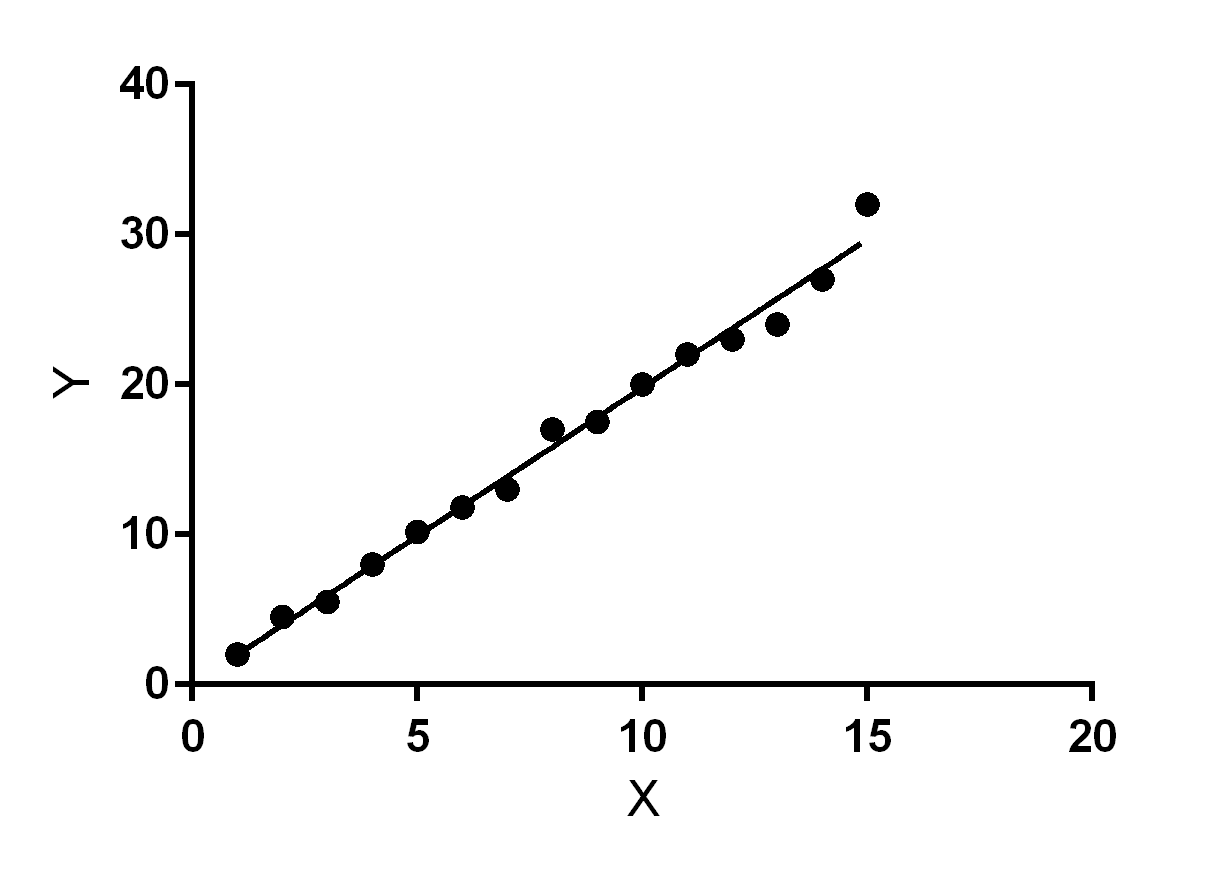
\includegraphics[scale=0.7]{Methods/Linear_regression.png}
      \end{center}
      \caption{Example linear regression}
      \label{fig:linear_regression}
  \end{figure}

  \par The way the independent variables are chosen is usually done by measuring the correlation coefficients between available features in a
  dataset and the target feature and then selecting the features having a high correlation coefficient. Depending on the problem setting, other features can be also considered 
  based on domain knowledge, especially when dealing with a mechanical system as in the case of this work. A good example of this would be the incorporation of 
  the ambient temperature measurement as an input feature---even if it does not highly correlate with the target feature---to make sure that your model generalizes, when 
  trying to predict a component's temperature throughout the year, by considering the effect of seasonality 
  (temperatures are expected to be higher in summer than in winter).\\
  In this work, we selected input features based on both domain knowledge and correlation coefficients. We used Kendall's method to measure the rank correlation \cite{Kendall}.
  In contrast to Pearson's correlation coefficient, Kendall's rank correlation can capture both linear and non-linear dependency between two variables by 
  measuring the monotonic relationship. In addition to that, variables don't have to be normally distributed when using Kendall's method.

\subsection{Deep learning}
  Although multiple linear regression models are capable of fitting the data with high accuracy in many applications (e.g., \cite{Linear_Regression_Example_1}), they are,
  by definition, not capable of capturing more complex non-linear dependencies. In addition to that, linear regression may not be appropriate when there are a significant 
  number of independent variables. Deep learning may be a better approach in these situations.\\
  After obtaining better results with it (see \ref{exp:I}), we decided to train the normal behavior models
  on a feed-forward neural network (for a comprehensive review of deep learning and neural networks, see \cite{Deep_Learning}) having the architecture shown 
  in fig. \ref{fig:MLP}.

  \begin{figure}[!htbp]
    \begin{center}
      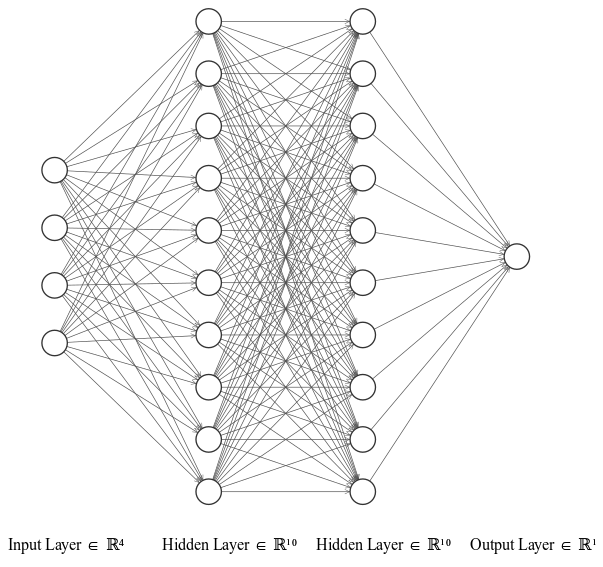
\includegraphics[scale=0.4]{Methods/MLP_cropped.png}
    \end{center}
    \caption{Architecture of normal behavior neural network model used in this work. \\
    \emph{P.S.: The input layer shape will vary based on the experiment and the number of input features.}}
    \label{fig:MLP}
  \end{figure}
  
\section{Log analysis}
In this section, we will describe the different approaches we propose to utilize SCADA log messages and incorporate them into normal behavior models.\\
In summary, we introduce three different ways for utilizing SCADA log messages: Extracting input features for normal behavior models, Data filtering, and Visualization of warnings.
We will explain each approach in depth.

\subsection{Extracting input features}
  Most machine-learning architectures can only work with vector-shaped numerical inputs. Given that there are limited resources in the research field on how to generate 
  numerical vectors from wind turbine SCADA system logs (see \ref{chap:soa}), we came up with two methods that were proven capable of not only generating input features for 
  machine-learning normal behavior models but also improving their accuracy (see \ref{chap:experiments}): 1. our Novel method based on domain knowledge and 
  2. Utilizing an open-source framework for analyzing log data called LogPAI. We will discuss each method in detail.

  \subsubsection{Novel method}
    \textbf{Background:}\\
    We scanned through the different log messages available in the dataset looking for information that reflects the turbine state and might help the normal behavior model 
    fit the data more accurately. Since normal behavior models monitor the state of a component by monitoring its temperature, we narrowed the search down to operation and system logs
    that reflect events causing a change of temperature in major components. We, then, ended up with the following list that we decided to analyze further:\\
    \begin{table}[H]
      \centering
      \begin{tabular}{|c|c|}
      \hline
       \textbf{Log text template} & \textbf{Log text sample}\\
       \hline
       Gen. ext. vent. \_, temp:\_\_\_\degree C & Gen. ext. vent. 2, temp:65\degree C \\
       Gen. int. vent. \_, temp:\_\_\_\degree C & Gen. ext. vent. 1, temp:50\degree C \\
       HV Trafo. vent. \_, temp:\_\_\_\degree C & HV Trafo. vent. 0, temp:2\degree C \\
       Nac.vent.\_, nac/gear:\_\_\_/\_\_\_\degree C & Nac.vent.3, nac/gear:43/ 54\degree C \\
  \hline
  \end{tabular}
  \caption{Logs}
      \label{tab:logs}
\end{table}
    Explain how the logs are filtered/selected, parsed and transformed into feature\\
    Since we're predicting temperatures, we focus on Vent logs only, because they have a clear impact on the temperature change of components (applying domain knowledge).\\
    \begin{figure}[!htbp]
      \begin{center}
        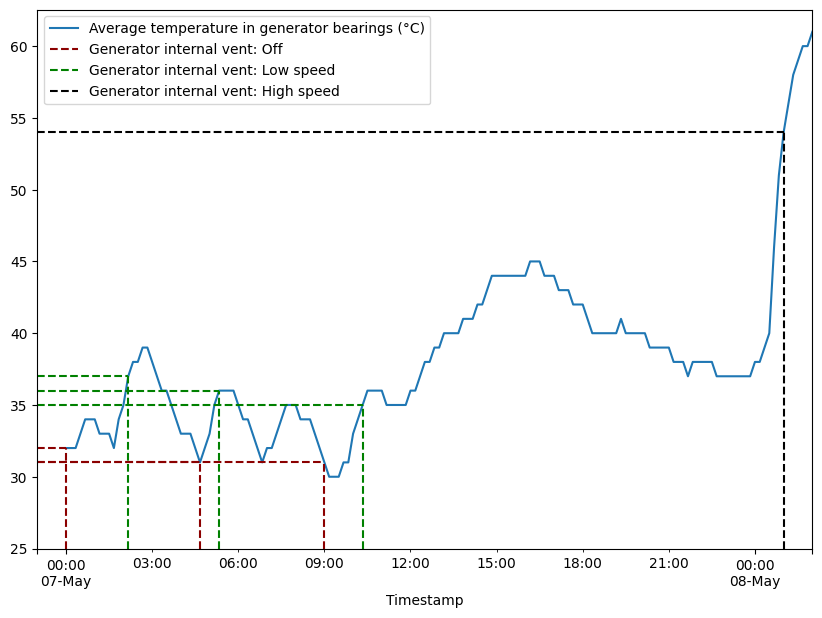
\includegraphics[scale=0.6]{Methods/Vent_Signals.png}
      \end{center}
      \caption{Sample control signals: Generator internal vent and its effect on the generator bearings temperature}
      \label{fig:vent}
    \end{figure}

  \subsubsection{Utilizing LogPAI}
    LogPAI (Log Analysis and Intelligence) is a study project and open-source platform for analyzing and managing log data \cite{LogPAI}. 
    Tsinghua University researchers started the project, which focuses on developing efficient algorithms and tools for log analysis, anomaly detection, and log data visualization.
    LogPAI includes a complete suite of log analysis and processing tools such as Logparser, Loglizer, and Logreduce. 
    These applications can assist users in preprocessing and parsing raw log data, detecting anomalies and patterns, and summarising log data concisely and understandably.\\

    TODO:\\
    1. Explain how the LogParser (Drain) works, what the format of the parsed log messages look like and why Drain -> Because online log parser\\
    2. Explain how LogLizer creates a feature from parsed logs

\subsection{Data filtering}
  TODO:\\
  Stoppages (log as filter)

\subsection{Visualization of warnings}
  TODO:\\
  Easy: look for any warning/alarm message (having the word "hot" or "high temperature") related to the target component (having the name of the component in the message) 
  and append to the anomaly on the operation dashboard

\section{Anomaly detection}
  TODO:\\
  Define anomalies (what is an anomaly in general?).\\
  Discuss anomaly detection methods used in other papers\\
  Argue why there's no standard way of defining/measuring an anomaly\\
  Describe the way our anomaly detection works.

\subsection{Alarms}
  TODO:\\
  Discuss the difference between Anomaly and alarm and why we wanna limit the number of alarms being sent to operators (false alarms are costly!)

\section{Summary}
TODO:\\
PUSH TO THE TOP//
Diagram of all methods put together: ML model + log feature + Anomaly detection + Alarms,...